\chapter{数据集与实际系统调研}
\label{sec:DataSetSystem}
\section{数据集调研}

本文调研与使用以下数据集用于评估提出的两种攻击方法的效果,通过模拟攻击评估重复数据删除中信息泄漏带来的安全隐患(参见\ref{sec:background})。

\subsection{FSL数据集}
\label{sec:fsl}
\begin{table}[!hbt]
    \caption{FSL数据集特征}
\small
\label{tab:FSL-dataset}
\centering
\begin{tabular}{|c|c|c|c|}
\hline
\multirow{2}{*}{\bf 类别} & \multicolumn{3}{c|}{\bf 备份中的特征} \\
\cline{2-4}
    & \#逻辑数据块数(百万) & \#唯一数据块数(百万) & 近似逻辑大小(GB)\\
\hline
User004  & 1.0-1.3 & 0.7-0.9 & 10GB/备份$\times$ 14个\\
\cline{1-4}
User007 &  3.5-5.2 & 2.3-3.6 & 39GB/备份 $\times$ 14个\\
\cline{1-4}
User012 &  25.0-26.4 & 8.9-9.7 & 244GB/备份 $\times$ 14个\\
\cline{1-4}
User013 &  1.8-5.7 & 1.2-4.2 & 22GB/备份 $\times$ 14个\\
\cline{1-4}
User015 &  13.4-20.5 & 9.0-11.0 & 158GB/备份 $\times$ 14个\\
\cline{1-4}
User028 &  6.0-10.3 & 3.5-6.8 & 77GB/备份 $\times$ 14个\\
\hline
\end{tabular}
\end{table}

表\ref{tab:FSL-dataset}总结了FSL实验数据集的相关特征信息,其中\#逻辑数据块数 和 \#唯一数据块数表示每个实验快照中逻辑数据块数量和具有唯一性的数据块数量。

此数据集由Stony Brook大学的文件系统和存储实验室(FSL)收集\citing{sun2016long,FSL14,sun2018cluster}。本文使用fslhomes快照进行实验,每个快照包括48位数据块哈希的有序列表,这些哈希是由平均大小为8KB的可变大小分块生成的,以及相应的元数据信息(例如,数据块大小、文件名、扩展名等)。本文从2013年1月22日到5月21日选择快照,并选择在整个持续时间内具有完整每日快照的六个用户(即User004,User007,User012,User013,User015和User028)用于后续实验分析。本文以周为单位选取备份数据,因此为每个用户选出14个每周完整备份。

\subsection{VM数据集}
\label{sec:vm}
\begin{table}[!hbt]
    \caption{VM数据集特征}
\small
\label{tab:VM-dataset}
\renewcommand{\arraystretch}{1.2}
\vspace{-3pt}
\centering
\begin{tabular}{|c|c|c|c|}
\hline
\multirow{2}{*}{\bf 类别} & \multicolumn{3}{c|}{\bf 备份中的特征} \\
\cline{2-4}
    & \#逻辑数据块数(百万) & \#唯一数据块数(百万) & 近似逻辑大小(GB)\\

\hline
User1  &  \multirow{6}{*}{2.6} & $\sim$0.9 & 25GB/备份 $\times$ 13 个 \\
\cline{1-1}
\cline{3-4}
User2 &  & 1.1-1.3 & 28GB/备份 $\times$ 13 个\\
\cline{1-1}
\cline{3-4}
User3 &  & 0.9-1.1 & 26GB/备份 $\times$ 13 个\\
\cline{1-1}
\cline{3-4}
User4 &  & $\sim$0.9 & 25GB/备份 $\times$ 13 个\\
\cline{1-1}
\cline{3-4}
User5 &  & 0.9-1.0 & 25GB/备份 $\times$ 13 个\\
\cline{1-1}
\cline{3-4}
User6 &  & 0.9-1.1 & 27GB/备份 $\times$ 13 个\\
\hline
\end{tabular} 
\end{table}

表\ref{tab:VM-dataset}总结了VM实验数据集的相关特征信息,其中\#逻辑数据块数 和 \#唯一数据块数表示每个实验快照中逻辑数据块数量和具有唯一性的数据块数量。由于所有的VM映像都具有10GB的固定大小,因此其具有相同数量的逻辑块。。

此数据集是从某大学2014年春季的编程课程中收集的。原始数据集包括为课程中注册的学生提供的大量VM镜像快照,每个快照的大小固定为10GB,每个快照中的数据用固定大小为4KB的数据块通过SHA-1算法计算得到的哈希的列表表示。本文使用6个用户(即User1-User6)的数据,每个用户的数据由13个每周备份组成。

\subsection{MS数据集}
\label{sec:ubc-ms}
\begin{table}[!hbt]
    \caption{MS数据集特征}
\small
\label{tab:MS-dataset}
\renewcommand{\arraystretch}{1.2}
\vspace{-3pt}
\centering
\begin{tabular}{|c|c|c|c|}
\hline
\multirow{2}{*}{\bf 类别} & \multicolumn{3}{c|}{\bf 备份中的特征} \\
\cline{2-4}
    & \#逻辑数据块数(百万) & \#唯一数据块数(百万) & 近似逻辑大小(GB)\\

\hline
Win7  & 61.6-61.8 & 61.1-61.3 & 425GB/备份 $\times$ 4 个\\
\cline{1-4}
Serv-03 & 10.6-10.7 & 8.4-8.5 & 78GB/备份 $\times$ 4 个\\
\cline{1-4}
Serv-08 & $\sim$6.5 & $\sim$3.8 & 48GB/备份 $\times$ 4 个\\
\cline{1-4}
Vista-B &  $\sim$7.6 & $\sim$2.0 & 55GB/备份 $\times$ 4 个\\
\cline{1-4}
Vista-U &  $\sim$21.0 & $\sim$10.4 & 159GB/备份 $\times$ 4 个\\
\hline
\end{tabular}
\end{table}

表\ref{tab:MS-dataset}总结了MS实验数据集的相关特征信息,其中\#逻辑数据块数 和 \#唯一数据块数表示每个实验快照中逻辑数据块数量和具有唯一性的数据块数量。

此数据集由Microsoft\citing{meyer2012study}收集,并在SNIA\citing{ms}上公布。 原始数据集包含2009年9月5日至10月31日的Windows文件系统快照。每个快照由通过Rabin Fingerprinting\citing{rabin1981fingerprinting}获得的不同平均大小的40位数据块哈希表示。 本文使用以下类别的操作系统快照用于试验:Windows 7(Win7),Microsoft Windows Server 2003(Serv-03),Microsoft Windows Server 2008(Serv-08),Microsoft Windows Vista Business Edition( Vista-B)和Microsoft Windows Vista Ultimate Edition(Vista-U)。在每个类别中,选择四个快照(这些快照的平均数据块大小为8KB。 


\section{实际系统调研}
\subsection{SDFS}

SDFS\citing{SDFS}是一种分布式、可扩展的文件系统,旨在为应用程序提供具有较强灵活性的内联重复数据删除。该系统有两种部署方法:

\begin{itemize}
    \item \textbf{单节点配置}:实际运行时将数据存储在本地文件系统中。
    \item \textbf{多节点配置}:实际运行中将数据存储在远端存储服务商/服务器中。
\end{itemize}

\subsubsection{系统的整体结构}

\par SDFS系统的整体结构如下所示:

\begin{figure}[!htb]
    \small
    \centering
    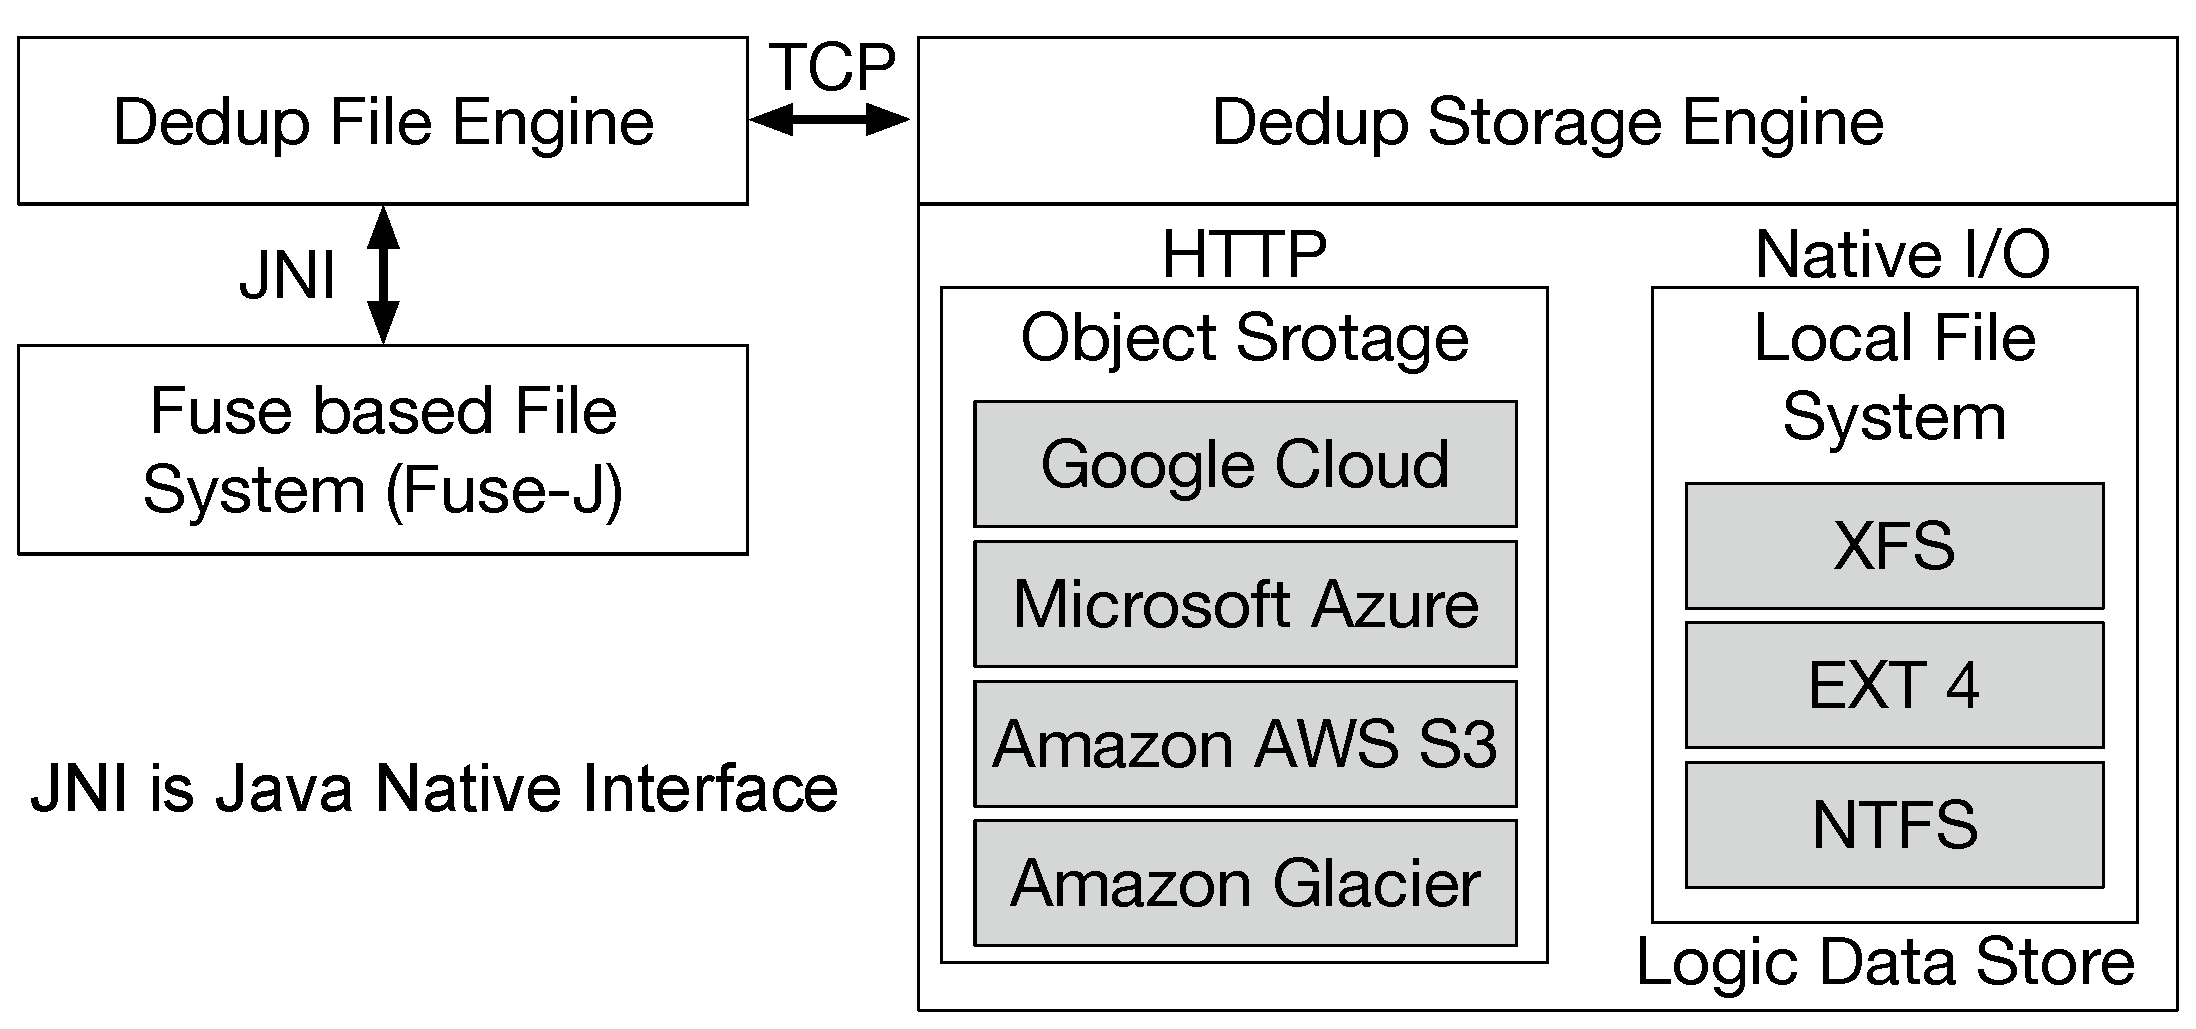
\includegraphics[width=11cm]{SDFS-Workflow}
    \caption{SDFS文件系统的运作流程} 
    \label{fig:SDFS-Workflow}
\end{figure}


该系统主要由以下四部分组成,其中Dedup File Engine和Dedup Storage Engine是SDFS系统的主要组件:

\begin{itemize}
    \item \textbf{Fuse Based File System (Fuse-J)}
    \item \textbf{Dedup File Engine}
    \item \textbf{Dedup Storage Engine}
    \item \textbf{Logic Data Store}
\end{itemize}


\subsubsection{Dedup File Engine}
本节将说明Dedup File Engine的工作原理以及相关的系统实现。Dedup File Engine的工作流程如下所示: 

\begin{figure}[!htb]
    \small
    \centering
    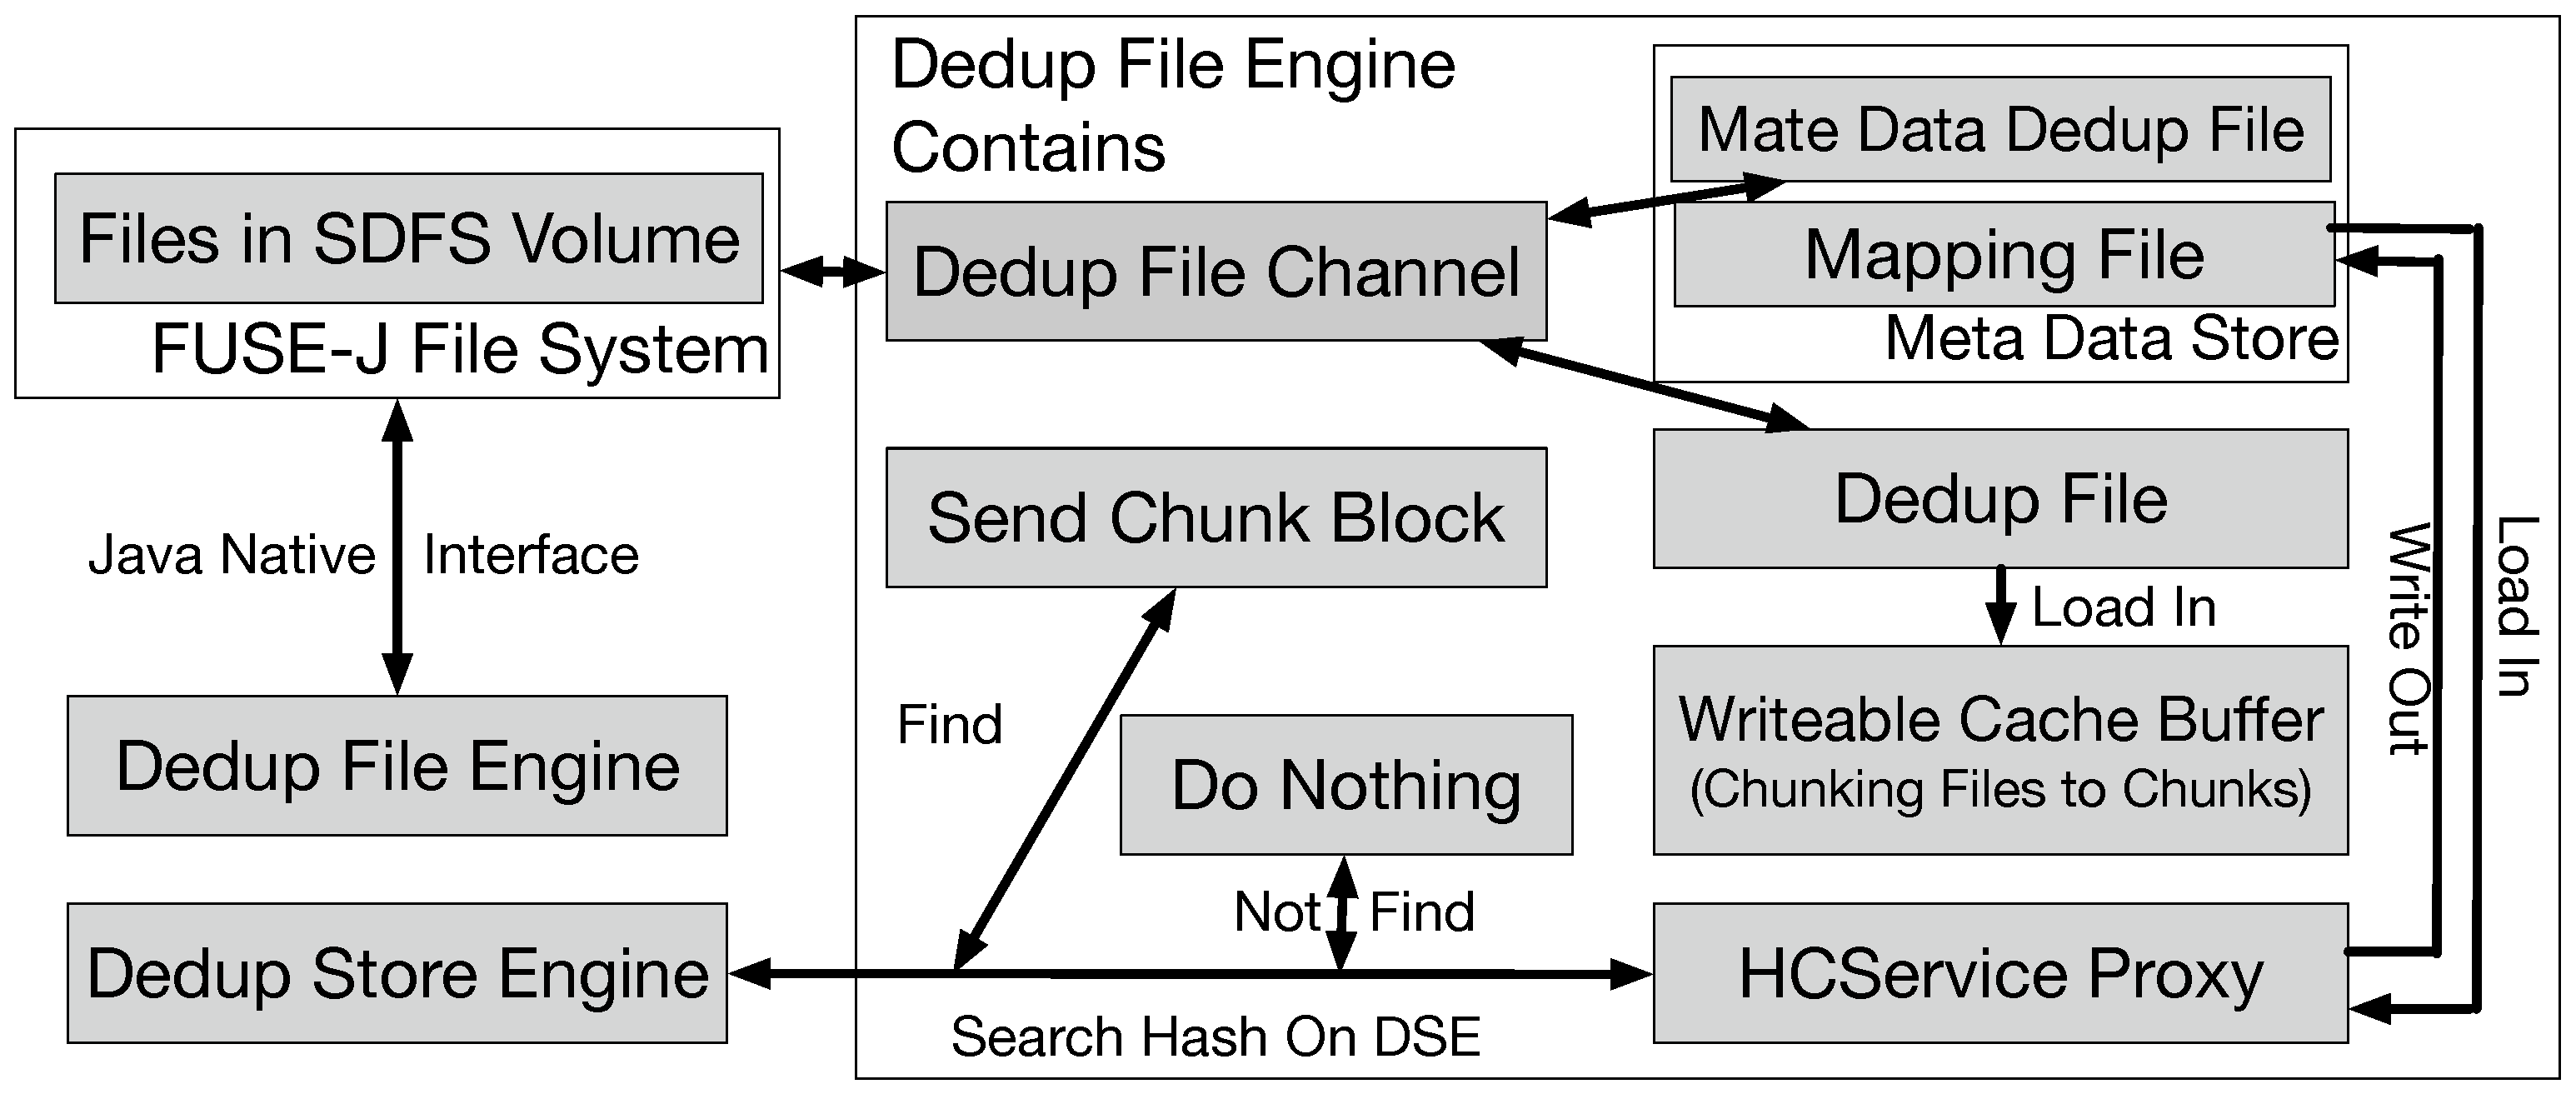
\includegraphics[width=11cm]{SDFS-DedupFileEngine.eps}
    \caption{SDFS文件系统的Dedup File Engine运作流程} 
    \label{fig:SDFS-DedupFileEngine}
\end{figure}

SDFS将Dedup File Engine通过Java Native Interface(JNI)连接到由FUSE-J驱动的实际文件系统的的卷,使得Dedup File Engine可以通过系统文件系统直接进行文件操作。

\textbf{Fuse-J Java Native Interface}

\begin{itemize}
    \item 文件统计和高级文件操作是通过获取和设置扩展文件属性(getfattr setfattr)来完成的。
    \item 每个挂载到SFDS的卷都拥有其独立的的Fuse-J接口和Dedup File Engine实例。
\end{itemize}

\textbf{Dedup File Channel}

本模块Fuse-J和DedupFile之间用于I/O命令的接口。该接口提供了一些方法(例如获取文件元数据/读取或写入文件)用于获取将进行重复数据删除的文件。

\textbf{Meta Data Store}


在SDFS文件系统中,文件通过两个不同的元数据进行表示,并将两种不同的元数据保存在两个不同的文件中。这两个文件分别为:

\begin{itemize}
    \item Meta Data Dedup File
    
    该文件用于存储进行重复数据删除的原始文件的文件属性元数据,包括文件大小、atime、ctime、acls以及指向关联映射文件的链接等。
    
    \item Mapping File

     该文件包含用于重复数据删除的文件的数据块记录列表,其存储了文件中每个数据块在原始文件中的位置、数据块是否具有唯一性、数据块的哈希值以及该数据块是否存储在远程服务器中。
\end{itemize}

\textbf{DedupFile}

该文件用于存储将要进行重复数据删除的文件的记录,其中的内容是挂载到SDFS文件系统的券中各个文件的哈希与完整文件路径与文件名的映射关系表。

\textbf{WritableCacheBuffer}

本数据结构包含一系列正在读取或写入的数据信息。在I/O活动期间,DedupFile会缓存其中的许多内容。在这部分中,SDFS使用SparseDedupFile类来处理writableCacheBuffer中的数据(即进行文件分块以获得获取逻辑数据块)。

SDFS支持两种数据块分块方法:固定大小的分块方法和Rabin可变大小数据块分块方法。

\textbf{HCService Proxy (HC == HashChunk)}

HCServiceProxy根据哈希的第一个字节(如果设置了多个Dedup Storage Engine)为当前数据块查找到适当的重复数据删除存储引擎。HCServiceProxy通过查询相应的Dedup File Engine以确定当前哈希所对应的数据块是否已存入存储系统(是否是重复的数据块),如果该数据块是重复的,则不进行任何操作,如果当前数据块是具有唯一性的,则将其加入存储系统中进行持久化存储。 


\subsubsection{Dedup Storage Engine}

Dedup Storage Engine(DSE)存储、检索和删除所有SDFS分割形成的数据块。重复数据删除存储引擎可以作为SDFS卷(单节点模式)的一部分运行,或在云端单独运行(多节点模式)。Dedup Storage Engine的运作流程如下所示: 

\begin{figure}[!htb]
    \small
    \centering
    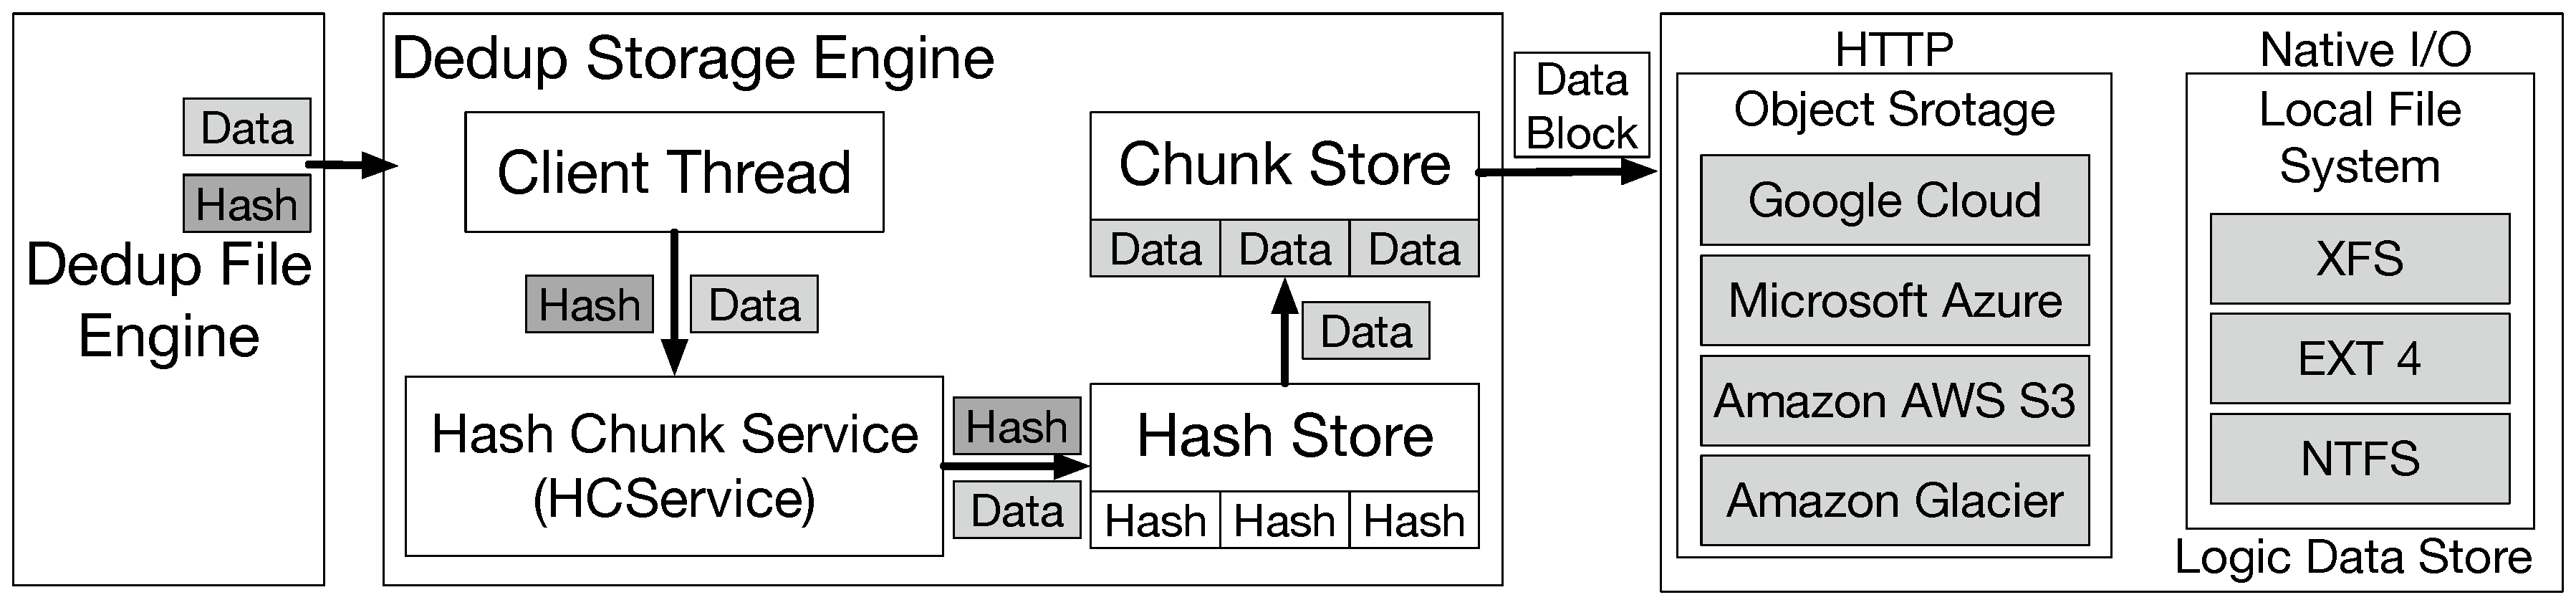
\includegraphics[width=\textwidth]{SDFS-DedupStorageEngine}
    \caption{SDFS文件系统的Dedup Storage Engine运作流程} 
    \label{fig:SDFS-DedupStorageEngine}
\end{figure}

\begin{enumerate}
    \item 客户端线程接收$WRITE\_HASH\_CMD$或$WRITE\_COMPRESSED\_CMD$信号并读取哈希和数据。
    \item 客户端线程将哈希传递给HashChunkService。
    \item HashChunkService将哈希和数据传递给适当的HashStore。
    \item HashStore存储哈希并将数据发送到指定的ChunkStore。
    \item ChunkStore存储数据。
\end{enumerate}

DES由2个基本组件组成:

\textbf{HashStore}

HashStore用于存储所有数据块的哈希与其对应的逻辑数据的存储位置。

\textbf{ChunkStore}

ChunkStore负责存储和检索与特定哈希相匹配的数据块原始逻辑数据。

\begin{itemize}
    \item 本地数据块存储
    \begin{itemize}
        \item 单文件数据块存储:将所有数据块写入一个文件中(文件大小与数据块总量有关)。
        \item 基于文件的数据块存储:将所有数据块依次写入固定大小的文件中。
    \end{itemize}
    \item 远程数据块存储
    \begin{itemize}
        \item Amazon S3
        \item Microsoft Azure
        \item Google Cloud
    \end{itemize}
\end{itemize}

\subsubsection{SDFS文件系统调研总结}

SDFS文件系统提供了商业使用级别的(加密)重复数据删除,但其中重复数据删除工作均先进行文件内的重复数据删除,再进行文件间的重复数据删除。其中的数据块处理顺序随机,不会发生数据块逻辑顺序信息的泄漏,因此可以防范本文提出的第一种攻击方法(基于分布的频率分析攻击方法)。但本文提出的第二种攻击手段在SDFS中仍然可以发挥作用。

\subsection{Destor}

Destor\citing{fu2015design}是重复数据删除的评估平台,其包含了大量重复数据删除中常用的方法,可以用于常用重复数据删除的方法测试与应用效果模拟评估。系统原型中包含的主要特征有:

\begin{itemize}
    \item 基于容器的数据块存储。
    \item 数据块级的管道通信。
    \item 三种重复数据删除方案:
    \begin{itemize}
        \item 基于固定大小的数据块分块的重复数据删除。
        \item 基于内容定义数据块分块方法的重复数据删除。
        \item 近似的文件级重复数据删除。
    \end{itemize}
    \item 多种文件重写算法:CFL、CBR、CAP和HAR等。
    \item 多种文件还原算法:LRU、最优替换算法和前滚组装。
\end{itemize}

\subsubsection{Destor系统原型调研总结}

Destor不同与商业化的SDFS文件系统,该系统原型是重复数据删除领域中著名的重复数据删除工具集合与样例。系统中的数据块处理是按照原有逻辑明文数据块的逻辑顺序进行的,因此会受到本文提出的两种攻击方法的威胁。

\section{本章小结}
本章介绍了本文用于评估攻击效果的三种真实世界数据集的来源和基本信息,以及两种现有重复数据删除系统的相关调研工作。
